\documentclass[1p]{elsarticle_modified}
%\bibliographystyle{elsarticle-num}

%\usepackage[colorlinks]{hyperref}
%\usepackage{abbrmath_seonhwa} %\Abb, \Ascr, \Acal ,\Abf, \Afrak
\usepackage{amsfonts}
\usepackage{amssymb}
\usepackage{amsmath}
\usepackage{amsthm}
\usepackage{scalefnt}
\usepackage{amsbsy}
\usepackage{kotex}
\usepackage{caption}
\usepackage{subfig}
\usepackage{color}
\usepackage{graphicx}
\usepackage{xcolor} %% white, black, red, green, blue, cyan, magenta, yellow
\usepackage{float}
\usepackage{setspace}
\usepackage{hyperref}

\usepackage{tikz}
\usetikzlibrary{arrows}

\usepackage{multirow}
\usepackage{array} % fixed length table
\usepackage{hhline}

%%%%%%%%%%%%%%%%%%%%%
\makeatletter
\renewcommand*\env@matrix[1][\arraystretch]{%
	\edef\arraystretch{#1}%
	\hskip -\arraycolsep
	\let\@ifnextchar\new@ifnextchar
	\array{*\c@MaxMatrixCols c}}
\makeatother %https://tex.stackexchange.com/questions/14071/how-can-i-increase-the-line-spacing-in-a-matrix
%%%%%%%%%%%%%%%

\usepackage[normalem]{ulem}

\newcommand{\msout}[1]{\ifmmode\text{\sout{\ensuremath{#1}}}\else\sout{#1}\fi}
%SOURCE: \msout is \stkout macro in https://tex.stackexchange.com/questions/20609/strikeout-in-math-mode

\newcommand{\cancel}[1]{
	\ifmmode
	{\color{red}\msout{#1}}
	\else
	{\color{red}\sout{#1}}
	\fi
}

\newcommand{\add}[1]{
	{\color{blue}\uwave{#1}}
}

\newcommand{\replace}[2]{
	\ifmmode
	{\color{red}\msout{#1}}{\color{blue}\uwave{#2}}
	\else
	{\color{red}\sout{#1}}{\color{blue}\uwave{#2}}
	\fi
}

\newcommand{\Sol}{\mathcal{S}} %segment
\newcommand{\D}{D} %diagram
\newcommand{\A}{\mathcal{A}} %arc


%%%%%%%%%%%%%%%%%%%%%%%%%%%%%5 test

\def\sl{\operatorname{\textup{SL}}(2,\Cbb)}
\def\psl{\operatorname{\textup{PSL}}(2,\Cbb)}
\def\quan{\mkern 1mu \triangleright \mkern 1mu}

\theoremstyle{definition}
\newtheorem{thm}{Theorem}[section]
\newtheorem{prop}[thm]{Proposition}
\newtheorem{lem}[thm]{Lemma}
\newtheorem{ques}[thm]{Question}
\newtheorem{cor}[thm]{Corollary}
\newtheorem{defn}[thm]{Definition}
\newtheorem{exam}[thm]{Example}
\newtheorem{rmk}[thm]{Remark}
\newtheorem{alg}[thm]{Algorithm}

\newcommand{\I}{\sqrt{-1}}
\begin{document}

%\begin{frontmatter}
%
%\title{Boundary parabolic representations of knots up to 8 crossings}
%
%%% Group authors per affiliation:
%\author{Yunhi Cho} 
%\address{Department of Mathematics, University of Seoul, Seoul, Korea}
%\ead{yhcho@uos.ac.kr}
%
%
%\author{Seonhwa Kim} %\fnref{s_kim}}
%\address{Center for Geometry and Physics, Institute for Basic Science, Pohang, 37673, Korea}
%\ead{ryeona17@ibs.re.kr}
%
%\author{Hyuk Kim}
%\address{Department of Mathematical Sciences, Seoul National University, Seoul 08826, Korea}
%\ead{hyukkim@snu.ac.kr}
%
%\author{Seokbeom Yoon}
%\address{Department of Mathematical Sciences, Seoul National University, Seoul, 08826,  Korea}
%\ead{sbyoon15@snu.ac.kr}
%
%\begin{abstract}
%We find all boundary parabolic representation of knots up to 8 crossings.
%
%\end{abstract}
%\begin{keyword}
%    \MSC[2010] 57M25 
%\end{keyword}
%
%\end{frontmatter}

%\linenumbers
%\tableofcontents
%
\newcommand\colored[1]{\textcolor{white}{\rule[-0.35ex]{0.8em}{1.4ex}}\kern-0.8em\color{red} #1}%
%\newcommand\colored[1]{\textcolor{white}{ #1}\kern-2.17ex	\textcolor{white}{ #1}\kern-1.81ex	\textcolor{white}{ #1}\kern-2.15ex\color{red}#1	}

{\Large $\underline{12n_{0681}~(K12n_{0681})}$}

\setlength{\tabcolsep}{10pt}
\renewcommand{\arraystretch}{1.6}
\vspace{1cm}\begin{tabular}{m{100pt}>{\centering\arraybackslash}m{274pt}}
\multirow{5}{120pt}{
	\centering
	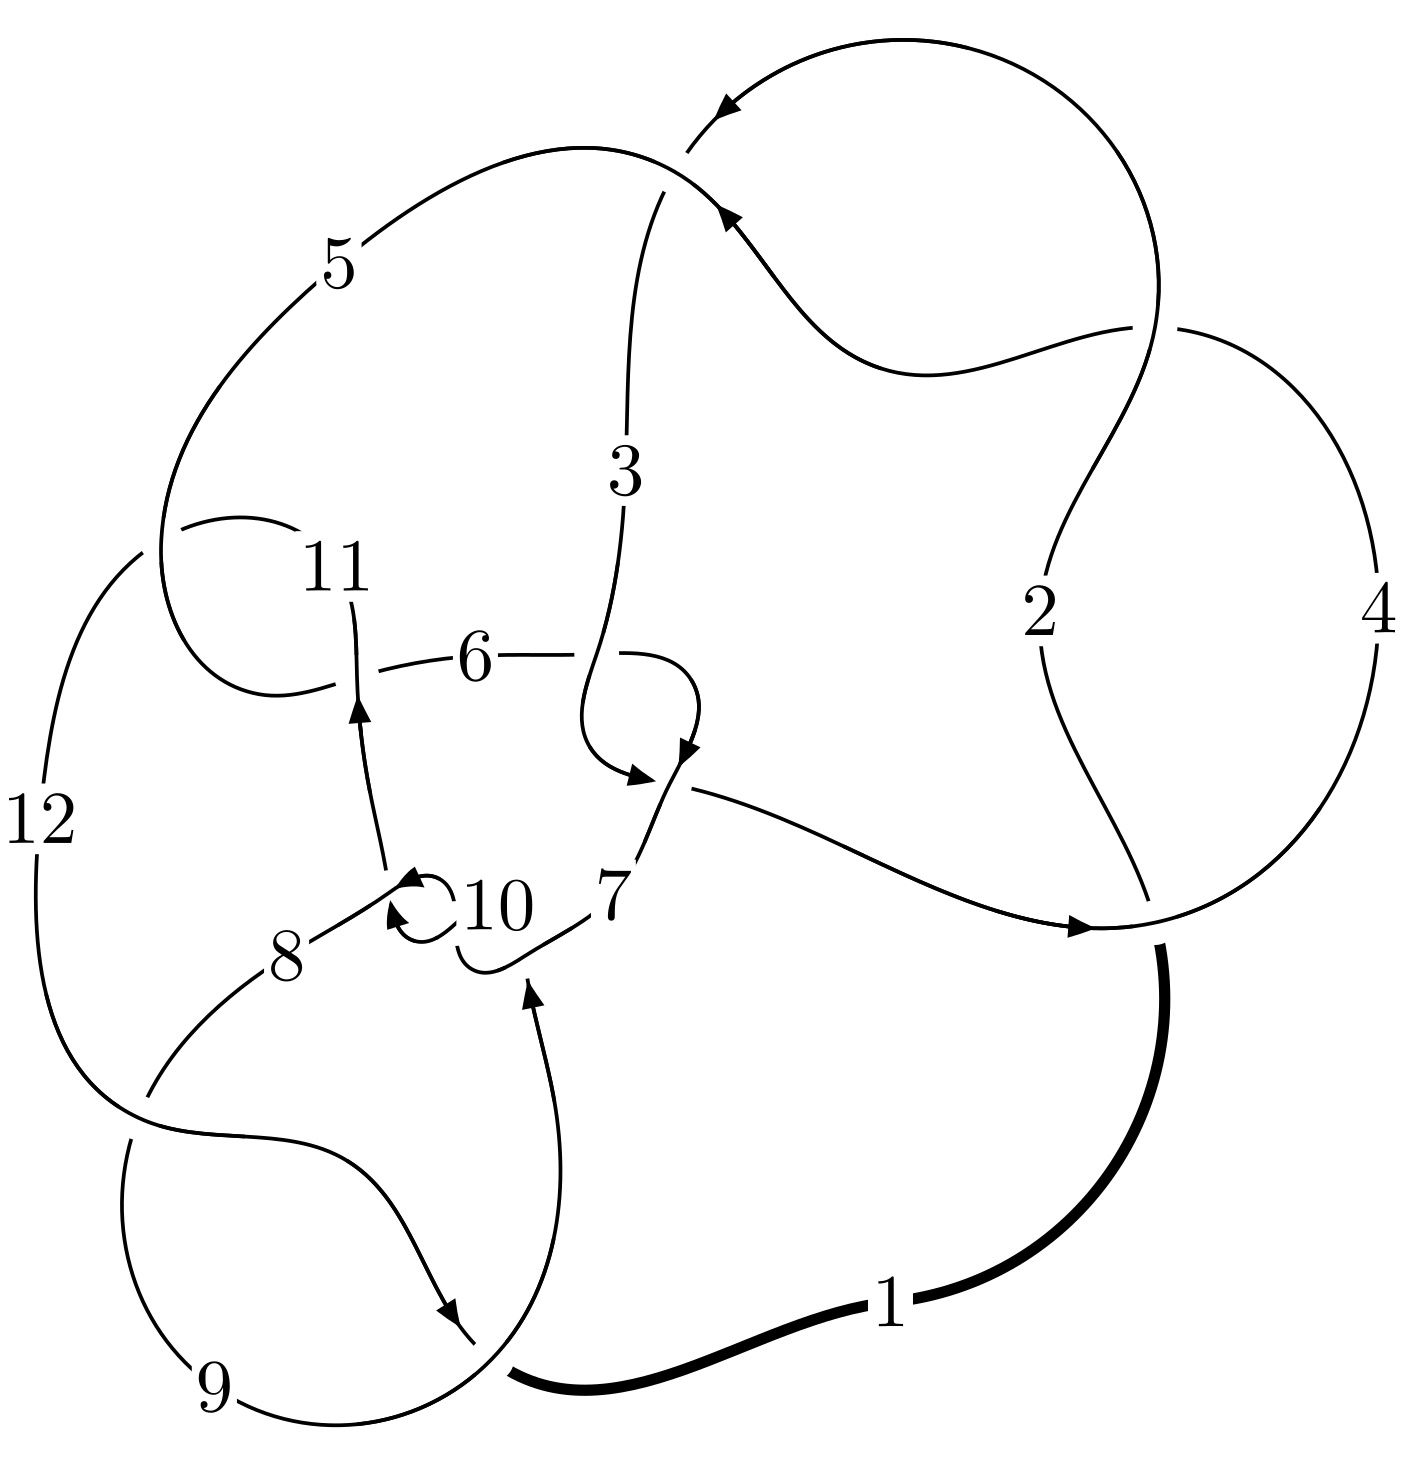
\includegraphics[width=112pt]{../../../GIT/diagram.site/Diagrams/png/2770_12n_0681.png}\\
\ \ \ A knot diagram\footnotemark}&
\allowdisplaybreaks
\textbf{Linearized knot diagam} \\
\cline{2-2}
 &
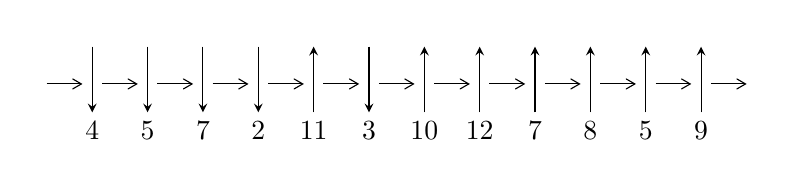
\begin{tikzpicture}[x=20pt, y=17pt]
	% nodes
	\node (C0) at (0, 0) {};
	\node (C1) at (1, 0) {};
	\node (C1U) at (1, +1) {};
	\node (C1D) at (1, -1) {4};

	\node (C2) at (2, 0) {};
	\node (C2U) at (2, +1) {};
	\node (C2D) at (2, -1) {5};

	\node (C3) at (3, 0) {};
	\node (C3U) at (3, +1) {};
	\node (C3D) at (3, -1) {7};

	\node (C4) at (4, 0) {};
	\node (C4U) at (4, +1) {};
	\node (C4D) at (4, -1) {2};

	\node (C5) at (5, 0) {};
	\node (C5U) at (5, +1) {};
	\node (C5D) at (5, -1) {11};

	\node (C6) at (6, 0) {};
	\node (C6U) at (6, +1) {};
	\node (C6D) at (6, -1) {3};

	\node (C7) at (7, 0) {};
	\node (C7U) at (7, +1) {};
	\node (C7D) at (7, -1) {10};

	\node (C8) at (8, 0) {};
	\node (C8U) at (8, +1) {};
	\node (C8D) at (8, -1) {12};

	\node (C9) at (9, 0) {};
	\node (C9U) at (9, +1) {};
	\node (C9D) at (9, -1) {7};

	\node (C10) at (10, 0) {};
	\node (C10U) at (10, +1) {};
	\node (C10D) at (10, -1) {8};

	\node (C11) at (11, 0) {};
	\node (C11U) at (11, +1) {};
	\node (C11D) at (11, -1) {5};

	\node (C12) at (12, 0) {};
	\node (C12U) at (12, +1) {};
	\node (C12D) at (12, -1) {9};
	\node (C13) at (13, 0) {};

	% arrows
	\draw[->,>={angle 60}]
	(C0) edge (C1) (C1) edge (C2) (C2) edge (C3) (C3) edge (C4) (C4) edge (C5) (C5) edge (C6) (C6) edge (C7) (C7) edge (C8) (C8) edge (C9) (C9) edge (C10) (C10) edge (C11) (C11) edge (C12) (C12) edge (C13) ;	\draw[->,>=stealth]
	(C1U) edge (C1D) (C2U) edge (C2D) (C3U) edge (C3D) (C4U) edge (C4D) (C5D) edge (C5U) (C6U) edge (C6D) (C7D) edge (C7U) (C8D) edge (C8U) (C9D) edge (C9U) (C10D) edge (C10U) (C11D) edge (C11U) (C12D) edge (C12U) ;
	\end{tikzpicture} \\
\hhline{~~} \\& 
\textbf{Solving Sequence} \\ \cline{2-2} 
 &
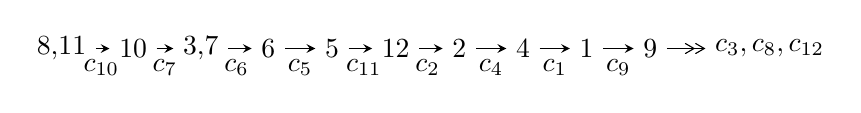
\begin{tikzpicture}[x=23pt, y=7pt]
	% node
	\node (A0) at (-1/8, 0) {8,11};
	\node (A1) at (1, 0) {10};
	\node (A2) at (33/16, 0) {3,7};
	\node (A3) at (25/8, 0) {6};
	\node (A4) at (33/8, 0) {5};
	\node (A5) at (41/8, 0) {12};
	\node (A6) at (49/8, 0) {2};
	\node (A7) at (57/8, 0) {4};
	\node (A8) at (65/8, 0) {1};
	\node (A9) at (73/8, 0) {9};
	\node (C1) at (1/2, -1) {$c_{10}$};
	\node (C2) at (3/2, -1) {$c_{7}$};
	\node (C3) at (21/8, -1) {$c_{6}$};
	\node (C4) at (29/8, -1) {$c_{5}$};
	\node (C5) at (37/8, -1) {$c_{11}$};
	\node (C6) at (45/8, -1) {$c_{2}$};
	\node (C7) at (53/8, -1) {$c_{4}$};
	\node (C8) at (61/8, -1) {$c_{1}$};
	\node (C9) at (69/8, -1) {$c_{9}$};
	\node (A10) at (11, 0) {$c_{3},c_{8},c_{12}$};

	% edge
	\draw[->,>=stealth]	
	(A0) edge (A1) (A1) edge (A2) (A2) edge (A3) (A3) edge (A4) (A4) edge (A5) (A5) edge (A6) (A6) edge (A7) (A7) edge (A8) (A8) edge (A9) ;
	\draw[->>,>={angle 60}]	
	(A9) edge (A10);
\end{tikzpicture} \\ 

\end{tabular} \\

\footnotetext{
The image of knot diagram is generated by the software ``\textbf{Draw programme}" developed by Andrew Bartholomew(\url{http://www.layer8.co.uk/maths/draw/index.htm\#Running-draw}), where we modified some parts for our purpose(\url{https://github.com/CATsTAILs/LinksPainter}).
}\phantom \\ \newline 
\centering \textbf{Ideals for irreducible components\footnotemark of $X_{\text{par}}$} 
 
\begin{align*}
I^u_{1}&=\langle 
-1.29319\times10^{25} u^{26}-8.14562\times10^{25} u^{25}+\cdots+2.10275\times10^{26} b+1.50746\times10^{26},\\
\phantom{I^u_{1}}&\phantom{= \langle  }9.51680\times10^{25} u^{26}+6.52825\times10^{26} u^{25}+\cdots+2.10275\times10^{26} a-7.67512\times10^{27},\;u^{27}+7 u^{26}+\cdots-65 u+1\rangle \\
I^u_{2}&=\langle 
- u^7-2 u^6+2 u^5+4 u^4-2 u^3- u^2+b+u-3,\;2 u^7+2 u^6-5 u^5-4 u^4+3 u^3+a+u+3,\\
\phantom{I^u_{2}}&\phantom{= \langle  }u^8+u^7-3 u^6-2 u^5+3 u^4+2 u-1\rangle \\
I^u_{3}&=\langle 
4 a^2+23 b-33 a+3,\;a^3-8 a^2+3 a-7,\;u-1\rangle \\
I^u_{4}&=\langle 
b-2 u+1,\;a+u+4,\;u^2+u-1\rangle \\
I^u_{5}&=\langle 
b+u,\;a- u-2,\;u^2+u-1\rangle \\
\\
\end{align*}
\raggedright * 5 irreducible components of $\dim_{\mathbb{C}}=0$, with total 42 representations.\\
\footnotetext{All coefficients of polynomials are rational numbers. But the coefficients are sometimes approximated in decimal forms when there is not enough margin.}
\newpage
\renewcommand{\arraystretch}{1}
\centering \section*{I. $I^u_{1}= \langle -1.29\times10^{25} u^{26}-8.15\times10^{25} u^{25}+\cdots+2.10\times10^{26} b+1.51\times10^{26},\;9.52\times10^{25} u^{26}+6.53\times10^{26} u^{25}+\cdots+2.10\times10^{26} a-7.68\times10^{27},\;u^{27}+7 u^{26}+\cdots-65 u+1 \rangle$}
\flushleft \textbf{(i) Arc colorings}\\
\begin{tabular}{m{7pt} m{180pt} m{7pt} m{180pt} }
\flushright $a_{8}=$&$\begin{pmatrix}0\\u\end{pmatrix}$ \\
\flushright $a_{11}=$&$\begin{pmatrix}1\\0\end{pmatrix}$ \\
\flushright $a_{10}=$&$\begin{pmatrix}1\\u^2\end{pmatrix}$ \\
\flushright $a_{3}=$&$\begin{pmatrix}-0.452588 u^{26}-3.10462 u^{25}+\cdots-55.6935 u+36.5004\\0.0614998 u^{26}+0.387379 u^{25}+\cdots+3.33121 u-0.716900\end{pmatrix}$ \\
\flushright $a_{7}=$&$\begin{pmatrix}- u\\- u^3+u\end{pmatrix}$ \\
\flushright $a_{6}=$&$\begin{pmatrix}-0.486093 u^{26}-3.57968 u^{25}+\cdots-55.8612 u+20.4963\\0.0646653 u^{26}+0.428826 u^{25}+\cdots+0.403387 u-0.357433\end{pmatrix}$ \\
\flushright $a_{5}=$&$\begin{pmatrix}-0.550758 u^{26}-4.00850 u^{25}+\cdots-56.2646 u+20.8537\\0.0646653 u^{26}+0.428826 u^{25}+\cdots+0.403387 u-0.357433\end{pmatrix}$ \\
\flushright $a_{12}=$&$\begin{pmatrix}-0.0697411 u^{26}-0.446921 u^{25}+\cdots-5.57659 u+8.05416\\-0.0811376 u^{26}-0.484277 u^{25}+\cdots+5.23091 u-0.200858\end{pmatrix}$ \\
\flushright $a_{2}=$&$\begin{pmatrix}-0.478778 u^{26}-3.47699 u^{25}+\cdots-53.7199 u+20.8543\\0.0459720 u^{26}+0.264293 u^{25}+\cdots-0.415707 u-0.385704\end{pmatrix}$ \\
\flushright $a_{4}=$&$\begin{pmatrix}-0.514677 u^{26}-3.50894 u^{25}+\cdots-55.7920 u+36.4942\\0.0496659 u^{26}+0.333051 u^{25}+\cdots+5.46117 u-0.741054\end{pmatrix}$ \\
\flushright $a_{1}=$&$\begin{pmatrix}0.0759051 u^{26}+0.518888 u^{25}+\cdots+8.57256 u-7.97571\\0.100287 u^{26}+0.631138 u^{25}+\cdots-2.83878 u+0.163326\end{pmatrix}$ \\
\flushright $a_{9}=$&$\begin{pmatrix}- u^2+1\\- u^4+2 u^2\end{pmatrix}$\\&\end{tabular}
\flushleft \textbf{(ii) Obstruction class $= -1$}\\~\\
\flushleft \textbf{(iii) Cusp Shapes $= -\frac{128221912491069143432166825}{210275241869650933749294956} u^{26}-\frac{1069012753234217659630964039}{210275241869650933749294956} u^{25}+\cdots-\frac{14132876007342110386546979695}{210275241869650933749294956} u-\frac{1802365230129749281114104905}{210275241869650933749294956}$}\\~\\
\newpage\renewcommand{\arraystretch}{1}
\flushleft \textbf{(iv) u-Polynomials at the component}\newline \\
\begin{tabular}{m{50pt}|m{274pt}}
Crossings & \hspace{64pt}u-Polynomials at each crossing \\
\hline $$\begin{aligned}c_{1},c_{2},c_{4}\end{aligned}$$&$\begin{aligned}
&u^{27}-12 u^{26}+\cdots-82 u-1
\end{aligned}$\\
\hline $$\begin{aligned}c_{3},c_{6}\end{aligned}$$&$\begin{aligned}
&u^{27}+4 u^{26}+\cdots+640 u-256
\end{aligned}$\\
\hline $$\begin{aligned}c_{5},c_{11}\end{aligned}$$&$\begin{aligned}
&u^{27}+3 u^{26}+\cdots-112 u+16
\end{aligned}$\\
\hline $$\begin{aligned}c_{7},c_{9},c_{10}\end{aligned}$$&$\begin{aligned}
&u^{27}+7 u^{26}+\cdots-65 u+1
\end{aligned}$\\
\hline $$\begin{aligned}c_{8},c_{12}\end{aligned}$$&$\begin{aligned}
&u^{27}-4 u^{26}+\cdots-36 u+8
\end{aligned}$\\
\hline
\end{tabular}\\~\\
\newpage\renewcommand{\arraystretch}{1}
\flushleft \textbf{(v) Riley Polynomials at the component}\newline \\
\begin{tabular}{m{50pt}|m{274pt}}
Crossings & \hspace{64pt}Riley Polynomials at each crossing \\
\hline $$\begin{aligned}c_{1},c_{2},c_{4}\end{aligned}$$&$\begin{aligned}
&y^{27}-46 y^{26}+\cdots+6314 y-1
\end{aligned}$\\
\hline $$\begin{aligned}c_{3},c_{6}\end{aligned}$$&$\begin{aligned}
&y^{27}-54 y^{26}+\cdots+5095424 y-65536
\end{aligned}$\\
\hline $$\begin{aligned}c_{5},c_{11}\end{aligned}$$&$\begin{aligned}
&y^{27}+25 y^{26}+\cdots+12928 y-256
\end{aligned}$\\
\hline $$\begin{aligned}c_{7},c_{9},c_{10}\end{aligned}$$&$\begin{aligned}
&y^{27}-15 y^{26}+\cdots+4023 y-1
\end{aligned}$\\
\hline $$\begin{aligned}c_{8},c_{12}\end{aligned}$$&$\begin{aligned}
&y^{27}+12 y^{26}+\cdots+7696 y-64
\end{aligned}$\\
\hline
\end{tabular}\\~\\
\newpage\flushleft \textbf{(vi) Complex Volumes and Cusp Shapes}
$$\begin{array}{c|c|c}  
\text{Solutions to }I^u_{1}& \I (\text{vol} + \sqrt{-1}CS) & \text{Cusp shape}\\
 \hline 
\begin{aligned}
u &= \phantom{-}0.989617\phantom{ +0.000000I} \\
a &= \phantom{-}9.38049\phantom{ +0.000000I} \\
b &= \phantom{-}0.408460\phantom{ +0.000000I}\end{aligned}
 & \phantom{-}0.561362\phantom{ +0.000000I} & \phantom{-}203.500\phantom{ +0.000000I} \\ \hline\begin{aligned}
u &= -1.035410 + 0.203452 I \\
a &= -0.415320 + 0.863420 I \\
b &= -0.33969 + 1.38997 I\end{aligned}
 & \phantom{-}4.69512 + 2.40532 I & \phantom{-}3.41247 + 6.32084 I \\ \hline\begin{aligned}
u &= -1.035410 - 0.203452 I \\
a &= -0.415320 - 0.863420 I \\
b &= -0.33969 - 1.38997 I\end{aligned}
 & \phantom{-}4.69512 - 2.40532 I & \phantom{-}3.41247 - 6.32084 I \\ \hline\begin{aligned}
u &= \phantom{-}1.035950 + 0.225932 I \\
a &= -0.376658 + 0.725229 I \\
b &= -0.061105 - 0.490914 I\end{aligned}
 & \phantom{-}1.156740 + 0.801856 I & \phantom{-}6.71973 + 0.16728 I \\ \hline\begin{aligned}
u &= \phantom{-}1.035950 - 0.225932 I \\
a &= -0.376658 - 0.725229 I \\
b &= -0.061105 + 0.490914 I\end{aligned}
 & \phantom{-}1.156740 - 0.801856 I & \phantom{-}6.71973 - 0.16728 I \\ \hline\begin{aligned}
u &= -0.231476 + 0.812947 I \\
a &= -1.010650 - 0.337430 I \\
b &= \phantom{-}0.147510 + 0.585443 I\end{aligned}
 & -2.46734 + 1.28188 I & \phantom{-}0.019660 - 0.966602 I \\ \hline\begin{aligned}
u &= -0.231476 - 0.812947 I \\
a &= -1.010650 + 0.337430 I \\
b &= \phantom{-}0.147510 - 0.585443 I\end{aligned}
 & -2.46734 - 1.28188 I & \phantom{-}0.019660 + 0.966602 I \\ \hline\begin{aligned}
u &= \phantom{-}0.707396\phantom{ +0.000000I} \\
a &= -4.75513\phantom{ +0.000000I} \\
b &= \phantom{-}0.0513464\phantom{ +0.000000I}\end{aligned}
 & -7.81649\phantom{ +0.000000I} & \phantom{-}57.8300\phantom{ +0.000000I} \\ \hline\begin{aligned}
u &= -1.305580 + 0.386979 I \\
a &= -0.110314 - 0.122910 I \\
b &= \phantom{-}0.073018 - 0.478334 I\end{aligned}
 & \phantom{-}1.16826 - 5.86191 I & \phantom{-}6.68570 + 1.60407 I \\ \hline\begin{aligned}
u &= -1.305580 - 0.386979 I \\
a &= -0.110314 + 0.122910 I \\
b &= \phantom{-}0.073018 + 0.478334 I\end{aligned}
 & \phantom{-}1.16826 + 5.86191 I & \phantom{-}6.68570 - 1.60407 I\\
 \hline 
 \end{array}$$\newpage$$\begin{array}{c|c|c}  
\text{Solutions to }I^u_{1}& \I (\text{vol} + \sqrt{-1}CS) & \text{Cusp shape}\\
 \hline 
\begin{aligned}
u &= -0.836004 + 1.095460 I \\
a &= -0.0688478 + 0.0584922 I \\
b &= -0.25035 + 1.73182 I\end{aligned}
 & -7.44159 - 1.29405 I & -1.37770 + 1.27497 I \\ \hline\begin{aligned}
u &= -0.836004 - 1.095460 I \\
a &= -0.0688478 - 0.0584922 I \\
b &= -0.25035 - 1.73182 I\end{aligned}
 & -7.44159 + 1.29405 I & -1.37770 - 1.27497 I \\ \hline\begin{aligned}
u &= \phantom{-}0.558394 + 0.255485 I \\
a &= \phantom{-}0.39540 + 1.82247 I \\
b &= -0.99845 - 1.93414 I\end{aligned}
 & -0.834252 + 0.150815 I & \phantom{-}17.5464 - 6.6365 I \\ \hline\begin{aligned}
u &= \phantom{-}0.558394 - 0.255485 I \\
a &= \phantom{-}0.39540 - 1.82247 I \\
b &= -0.99845 + 1.93414 I\end{aligned}
 & -0.834252 - 0.150815 I & \phantom{-}17.5464 + 6.6365 I \\ \hline\begin{aligned}
u &= -1.016510 + 0.945163 I \\
a &= \phantom{-}1.046130 - 0.262688 I \\
b &= -0.340400 - 0.098336 I\end{aligned}
 & -13.16990 - 3.53439 I & -0.41212 + 2.09406 I \\ \hline\begin{aligned}
u &= -1.016510 - 0.945163 I \\
a &= \phantom{-}1.046130 + 0.262688 I \\
b &= -0.340400 + 0.098336 I\end{aligned}
 & -13.16990 + 3.53439 I & -0.41212 - 2.09406 I \\ \hline\begin{aligned}
u &= -1.16800 + 0.91505 I \\
a &= \phantom{-}1.271790 - 0.556686 I \\
b &= -0.35535 - 1.77081 I\end{aligned}
 & -6.34499 - 6.08931 I & -0.21731 + 3.73020 I \\ \hline\begin{aligned}
u &= -1.16800 - 0.91505 I \\
a &= \phantom{-}1.271790 + 0.556686 I \\
b &= -0.35535 + 1.77081 I\end{aligned}
 & -6.34499 + 6.08931 I & -0.21731 - 3.73020 I \\ \hline\begin{aligned}
u &= \phantom{-}0.491518\phantom{ +0.000000I} \\
a &= -0.797650\phantom{ +0.000000I} \\
b &= \phantom{-}0.376982\phantom{ +0.000000I}\end{aligned}
 & \phantom{-}0.859867\phantom{ +0.000000I} & \phantom{-}11.9670\phantom{ +0.000000I} \\ \hline\begin{aligned}
u &= \phantom{-}0.06761 + 1.51979 I \\
a &= -0.239446 + 0.151266 I \\
b &= \phantom{-}0.28102 - 2.41058 I\end{aligned}
 & \phantom{-}18.5782 + 5.9421 I & -1.31050 - 2.20591 I\\
 \hline 
 \end{array}$$\newpage$$\begin{array}{c|c|c}  
\text{Solutions to }I^u_{1}& \I (\text{vol} + \sqrt{-1}CS) & \text{Cusp shape}\\
 \hline 
\begin{aligned}
u &= \phantom{-}0.06761 - 1.51979 I \\
a &= -0.239446 - 0.151266 I \\
b &= \phantom{-}0.28102 + 2.41058 I\end{aligned}
 & \phantom{-}18.5782 - 5.9421 I & -1.31050 + 2.20591 I \\ \hline\begin{aligned}
u &= -1.60127\phantom{ +0.000000I} \\
a &= \phantom{-}2.03965\phantom{ +0.000000I} \\
b &= \phantom{-}3.57318\phantom{ +0.000000I}\end{aligned}
 & \phantom{-}7.98804\phantom{ +0.000000I} & \phantom{-}43.0640\phantom{ +0.000000I} \\ \hline\begin{aligned}
u &= -1.55855 + 0.65683 I \\
a &= -1.03603 + 1.21486 I \\
b &= \phantom{-}0.57720 + 2.23959 I\end{aligned}
 & -15.7574 - 13.5083 I & \phantom{-}0.77209 + 5.37939 I \\ \hline\begin{aligned}
u &= -1.55855 - 0.65683 I \\
a &= -1.03603 - 1.21486 I \\
b &= \phantom{-}0.57720 - 2.23959 I\end{aligned}
 & -15.7574 + 13.5083 I & \phantom{-}0.77209 - 5.37939 I \\ \hline\begin{aligned}
u &= \phantom{-}1.68805 + 0.77291 I \\
a &= \phantom{-}0.823135 + 0.943566 I \\
b &= -0.10758 + 2.58327 I\end{aligned}
 & -16.0044 + 2.3695 I & \phantom{-0.000000 } 0 \\ \hline\begin{aligned}
u &= \phantom{-}1.68805 - 0.77291 I \\
a &= \phantom{-}0.823135 - 0.943566 I \\
b &= -0.10758 - 2.58327 I\end{aligned}
 & -16.0044 - 2.3695 I & \phantom{-0.000000 } 0 \\ \hline\begin{aligned}
u &= \phantom{-}0.0157914\phantom{ +0.000000I} \\
a &= \phantom{-}35.5742\phantom{ +0.000000I} \\
b &= -0.661597\phantom{ +0.000000I}\end{aligned}
 & -1.12664\phantom{ +0.000000I} & -9.59770\phantom{ +0.000000I}\\
 \hline 
 \end{array}$$\newpage\newpage\renewcommand{\arraystretch}{1}
\centering \section*{II. $I^u_{2}= \langle - u^7-2 u^6+2 u^5+4 u^4-2 u^3- u^2+b+u-3,\;2 u^7+2 u^6-5 u^5-4 u^4+3 u^3+a+u+3,\;u^8+u^7-3 u^6-2 u^5+3 u^4+2 u-1 \rangle$}
\flushleft \textbf{(i) Arc colorings}\\
\begin{tabular}{m{7pt} m{180pt} m{7pt} m{180pt} }
\flushright $a_{8}=$&$\begin{pmatrix}0\\u\end{pmatrix}$ \\
\flushright $a_{11}=$&$\begin{pmatrix}1\\0\end{pmatrix}$ \\
\flushright $a_{10}=$&$\begin{pmatrix}1\\u^2\end{pmatrix}$ \\
\flushright $a_{3}=$&$\begin{pmatrix}-2 u^7-2 u^6+5 u^5+4 u^4-3 u^3- u-3\\u^7+2 u^6-2 u^5-4 u^4+2 u^3+u^2- u+3\end{pmatrix}$ \\
\flushright $a_{7}=$&$\begin{pmatrix}- u\\- u^3+u\end{pmatrix}$ \\
\flushright $a_{6}=$&$\begin{pmatrix}- u\\- u^3+u\end{pmatrix}$ \\
\flushright $a_{5}=$&$\begin{pmatrix}u^3-2 u\\- u^3+u\end{pmatrix}$ \\
\flushright $a_{12}=$&$\begin{pmatrix}u^6-3 u^4+2 u^2+1\\- u^6+2 u^4- u^2\end{pmatrix}$ \\
\flushright $a_{2}=$&$\begin{pmatrix}-2 u^7-2 u^6+5 u^5+4 u^4-4 u^3+u-3\\u^7+2 u^6-2 u^5-4 u^4+3 u^3+u^2-2 u+3\end{pmatrix}$ \\
\flushright $a_{4}=$&$\begin{pmatrix}-2 u^7-2 u^6+5 u^5+4 u^4-3 u^3- u-3\\u^7+2 u^6-2 u^5-4 u^4+2 u^3+u^2- u+3\end{pmatrix}$ \\
\flushright $a_{1}=$&$\begin{pmatrix}- u^3+2 u\\u^3- u\end{pmatrix}$ \\
\flushright $a_{9}=$&$\begin{pmatrix}- u^2+1\\- u^4+2 u^2\end{pmatrix}$\\&\end{tabular}
\flushleft \textbf{(ii) Obstruction class $= 1$}\\~\\
\flushleft \textbf{(iii) Cusp Shapes $= 21 u^7+38 u^6-48 u^5-85 u^4+39 u^3+27 u^2-5 u+58$}\\~\\
\newpage\renewcommand{\arraystretch}{1}
\flushleft \textbf{(iv) u-Polynomials at the component}\newline \\
\begin{tabular}{m{50pt}|m{274pt}}
Crossings & \hspace{64pt}u-Polynomials at each crossing \\
\hline $$\begin{aligned}c_{1},c_{2}\end{aligned}$$&$\begin{aligned}
&(u-1)^8
\end{aligned}$\\
\hline $$\begin{aligned}c_{3},c_{6}\end{aligned}$$&$\begin{aligned}
&u^8
\end{aligned}$\\
\hline $$\begin{aligned}c_{4}\end{aligned}$$&$\begin{aligned}
&(u+1)^8
\end{aligned}$\\
\hline $$\begin{aligned}c_{5}\end{aligned}$$&$\begin{aligned}
&u^8+3 u^7+7 u^6+10 u^5+11 u^4+10 u^3+6 u^2+4 u+1
\end{aligned}$\\
\hline $$\begin{aligned}c_{7}\end{aligned}$$&$\begin{aligned}
&u^8- u^7-3 u^6+2 u^5+3 u^4-2 u-1
\end{aligned}$\\
\hline $$\begin{aligned}c_{8}\end{aligned}$$&$\begin{aligned}
&u^8+u^7- u^6-2 u^5+u^4+2 u^3-2 u-1
\end{aligned}$\\
\hline $$\begin{aligned}c_{9},c_{10}\end{aligned}$$&$\begin{aligned}
&u^8+u^7-3 u^6-2 u^5+3 u^4+2 u-1
\end{aligned}$\\
\hline $$\begin{aligned}c_{11}\end{aligned}$$&$\begin{aligned}
&u^8-3 u^7+7 u^6-10 u^5+11 u^4-10 u^3+6 u^2-4 u+1
\end{aligned}$\\
\hline $$\begin{aligned}c_{12}\end{aligned}$$&$\begin{aligned}
&u^8- u^7- u^6+2 u^5+u^4-2 u^3+2 u-1
\end{aligned}$\\
\hline
\end{tabular}\\~\\
\newpage\renewcommand{\arraystretch}{1}
\flushleft \textbf{(v) Riley Polynomials at the component}\newline \\
\begin{tabular}{m{50pt}|m{274pt}}
Crossings & \hspace{64pt}Riley Polynomials at each crossing \\
\hline $$\begin{aligned}c_{1},c_{2},c_{4}\end{aligned}$$&$\begin{aligned}
&(y-1)^8
\end{aligned}$\\
\hline $$\begin{aligned}c_{3},c_{6}\end{aligned}$$&$\begin{aligned}
&y^8
\end{aligned}$\\
\hline $$\begin{aligned}c_{5},c_{11}\end{aligned}$$&$\begin{aligned}
&y^8+5 y^7+11 y^6+6 y^5-17 y^4-34 y^3-22 y^2-4 y+1
\end{aligned}$\\
\hline $$\begin{aligned}c_{7},c_{9},c_{10}\end{aligned}$$&$\begin{aligned}
&y^8-7 y^7+19 y^6-22 y^5+3 y^4+14 y^3-6 y^2-4 y+1
\end{aligned}$\\
\hline $$\begin{aligned}c_{8},c_{12}\end{aligned}$$&$\begin{aligned}
&y^8-3 y^7+7 y^6-10 y^5+11 y^4-10 y^3+6 y^2-4 y+1
\end{aligned}$\\
\hline
\end{tabular}\\~\\
\newpage\flushleft \textbf{(vi) Complex Volumes and Cusp Shapes}
$$\begin{array}{c|c|c}  
\text{Solutions to }I^u_{2}& \I (\text{vol} + \sqrt{-1}CS) & \text{Cusp shape}\\
 \hline 
\begin{aligned}
u &= \phantom{-}1.180120 + 0.268597 I \\
a &= \phantom{-}1.23903 + 1.07030 I \\
b &= -0.281371 + 1.128550 I\end{aligned}
 & -0.604279 + 1.131230 I & \phantom{-}0.744211 + 0.553382 I \\ \hline\begin{aligned}
u &= \phantom{-}1.180120 - 0.268597 I \\
a &= \phantom{-}1.23903 - 1.07030 I \\
b &= -0.281371 - 1.128550 I\end{aligned}
 & -0.604279 - 1.131230 I & \phantom{-}0.744211 - 0.553382 I \\ \hline\begin{aligned}
u &= \phantom{-}0.108090 + 0.747508 I \\
a &= -0.188536 + 0.513699 I \\
b &= \phantom{-}0.208670 - 0.825203 I\end{aligned}
 & -3.80435 + 2.57849 I & -2.39106 - 4.72239 I \\ \hline\begin{aligned}
u &= \phantom{-}0.108090 - 0.747508 I \\
a &= -0.188536 - 0.513699 I \\
b &= \phantom{-}0.208670 + 0.825203 I\end{aligned}
 & -3.80435 - 2.57849 I & -2.39106 + 4.72239 I \\ \hline\begin{aligned}
u &= -1.37100\phantom{ +0.000000I} \\
a &= \phantom{-}0.942639\phantom{ +0.000000I} \\
b &= \phantom{-}0.829189\phantom{ +0.000000I}\end{aligned}
 & \phantom{-}4.85780\phantom{ +0.000000I} & \phantom{-}8.45210\phantom{ +0.000000I} \\ \hline\begin{aligned}
u &= -1.334530 + 0.318930 I \\
a &= -0.271933 + 0.551071 I \\
b &= \phantom{-}0.284386 + 0.605794 I\end{aligned}
 & \phantom{-}0.73474 - 6.44354 I & \phantom{-}0.47538 + 9.99765 I \\ \hline\begin{aligned}
u &= -1.334530 - 0.318930 I \\
a &= -0.271933 - 0.551071 I \\
b &= \phantom{-}0.284386 - 0.605794 I\end{aligned}
 & \phantom{-}0.73474 + 6.44354 I & \phantom{-}0.47538 - 9.99765 I \\ \hline\begin{aligned}
u &= \phantom{-}0.463640\phantom{ +0.000000I} \\
a &= -3.49976\phantom{ +0.000000I} \\
b &= \phantom{-}2.74744\phantom{ +0.000000I}\end{aligned}
 & -0.799899\phantom{ +0.000000I} & \phantom{-}60.8910\phantom{ +0.000000I}\\
 \hline 
 \end{array}$$\newpage\newpage\renewcommand{\arraystretch}{1}
\centering \section*{III. $I^u_{3}= \langle 4 a^2+23 b-33 a+3,\;a^3-8 a^2+3 a-7,\;u-1 \rangle$}
\flushleft \textbf{(i) Arc colorings}\\
\begin{tabular}{m{7pt} m{180pt} m{7pt} m{180pt} }
\flushright $a_{8}=$&$\begin{pmatrix}0\\1\end{pmatrix}$ \\
\flushright $a_{11}=$&$\begin{pmatrix}1\\0\end{pmatrix}$ \\
\flushright $a_{10}=$&$\begin{pmatrix}1\\1\end{pmatrix}$ \\
\flushright $a_{3}=$&$\begin{pmatrix}a\\-\frac{4}{23} a^2+\frac{33}{23} a-\frac{3}{23}\end{pmatrix}$ \\
\flushright $a_{7}=$&$\begin{pmatrix}-1\\0\end{pmatrix}$ \\
\flushright $a_{6}=$&$\begin{pmatrix}\frac{1}{23} a^2+\frac{9}{23} a-\frac{51}{23}\\-\frac{1}{23} a^2+\frac{14}{23} a-\frac{41}{23}\end{pmatrix}$ \\
\flushright $a_{5}=$&$\begin{pmatrix}\frac{2}{23} a^2-\frac{5}{23} a-\frac{10}{23}\\-\frac{1}{23} a^2+\frac{14}{23} a-\frac{41}{23}\end{pmatrix}$ \\
\flushright $a_{12}=$&$\begin{pmatrix}0\\-\frac{5}{23} a^2+\frac{47}{23} a-\frac{67}{23}\end{pmatrix}$ \\
\flushright $a_{2}=$&$\begin{pmatrix}\frac{1}{23} a^2+\frac{9}{23} a-\frac{5}{23}\\-\frac{1}{23} a^2+\frac{14}{23} a-\frac{41}{23}\end{pmatrix}$ \\
\flushright $a_{4}=$&$\begin{pmatrix}\frac{4}{23} a^2-\frac{10}{23} a+\frac{3}{23}\\-\frac{4}{23} a^2+\frac{33}{23} a-\frac{3}{23}\end{pmatrix}$ \\
\flushright $a_{1}=$&$\begin{pmatrix}0\\-\frac{5}{23} a^2+\frac{47}{23} a-\frac{67}{23}\end{pmatrix}$ \\
\flushright $a_{9}=$&$\begin{pmatrix}0\\1\end{pmatrix}$\\&\end{tabular}
\flushleft \textbf{(ii) Obstruction class $= 1$}\\~\\
\flushleft \textbf{(iii) Cusp Shapes $= -\frac{75}{23} a^2+\frac{314}{23} a-\frac{39}{23}$}\\~\\
\newpage\renewcommand{\arraystretch}{1}
\flushleft \textbf{(iv) u-Polynomials at the component}\newline \\
\begin{tabular}{m{50pt}|m{274pt}}
Crossings & \hspace{64pt}u-Polynomials at each crossing \\
\hline $$\begin{aligned}c_{1},c_{2}\end{aligned}$$&$\begin{aligned}
&u^3+u^2-1
\end{aligned}$\\
\hline $$\begin{aligned}c_{3}\end{aligned}$$&$\begin{aligned}
&u^3- u^2+2 u-1
\end{aligned}$\\
\hline $$\begin{aligned}c_{4}\end{aligned}$$&$\begin{aligned}
&u^3- u^2+1
\end{aligned}$\\
\hline $$\begin{aligned}c_{5}\end{aligned}$$&$\begin{aligned}
&u^3-3 u^2+2 u+1
\end{aligned}$\\
\hline $$\begin{aligned}c_{6}\end{aligned}$$&$\begin{aligned}
&u^3+u^2+2 u+1
\end{aligned}$\\
\hline $$\begin{aligned}c_{7}\end{aligned}$$&$\begin{aligned}
&(u+1)^3
\end{aligned}$\\
\hline $$\begin{aligned}c_{8},c_{12}\end{aligned}$$&$\begin{aligned}
&u^3
\end{aligned}$\\
\hline $$\begin{aligned}c_{9},c_{10}\end{aligned}$$&$\begin{aligned}
&(u-1)^3
\end{aligned}$\\
\hline $$\begin{aligned}c_{11}\end{aligned}$$&$\begin{aligned}
&u^3+3 u^2+2 u-1
\end{aligned}$\\
\hline
\end{tabular}\\~\\
\newpage\renewcommand{\arraystretch}{1}
\flushleft \textbf{(v) Riley Polynomials at the component}\newline \\
\begin{tabular}{m{50pt}|m{274pt}}
Crossings & \hspace{64pt}Riley Polynomials at each crossing \\
\hline $$\begin{aligned}c_{1},c_{2},c_{4}\end{aligned}$$&$\begin{aligned}
&y^3- y^2+2 y-1
\end{aligned}$\\
\hline $$\begin{aligned}c_{3},c_{6}\end{aligned}$$&$\begin{aligned}
&y^3+3 y^2+2 y-1
\end{aligned}$\\
\hline $$\begin{aligned}c_{5},c_{11}\end{aligned}$$&$\begin{aligned}
&y^3-5 y^2+10 y-1
\end{aligned}$\\
\hline $$\begin{aligned}c_{7},c_{9},c_{10}\end{aligned}$$&$\begin{aligned}
&(y-1)^3
\end{aligned}$\\
\hline $$\begin{aligned}c_{8},c_{12}\end{aligned}$$&$\begin{aligned}
&y^3
\end{aligned}$\\
\hline
\end{tabular}\\~\\
\newpage\flushleft \textbf{(vi) Complex Volumes and Cusp Shapes}
$$\begin{array}{c|c|c}  
\text{Solutions to }I^u_{3}& \I (\text{vol} + \sqrt{-1}CS) & \text{Cusp shape}\\
 \hline 
\begin{aligned}
u &= \phantom{-}1.00000\phantom{ +0.000000I} \\
a &= \phantom{-}0.135484 + 0.941977 I \\
b &= \phantom{-}0.215080 + 1.307140 I\end{aligned}
 & \phantom{-}4.66906 - 2.82812 I & \phantom{-}2.98758 + 12.02771 I \\ \hline\begin{aligned}
u &= \phantom{-}1.00000\phantom{ +0.000000I} \\
a &= \phantom{-}0.135484 - 0.941977 I \\
b &= \phantom{-}0.215080 - 1.307140 I\end{aligned}
 & \phantom{-}4.66906 + 2.82812 I & \phantom{-}2.98758 - 12.02771 I \\ \hline\begin{aligned}
u &= \phantom{-}1.00000\phantom{ +0.000000I} \\
a &= \phantom{-}7.72903\phantom{ +0.000000I} \\
b &= \phantom{-}0.569840\phantom{ +0.000000I}\end{aligned}
 & \phantom{-}0.531480\phantom{ +0.000000I} & -90.9750\phantom{ +0.000000I}\\
 \hline 
 \end{array}$$\newpage\newpage\renewcommand{\arraystretch}{1}
\centering \section*{IV. $I^u_{4}= \langle b-2 u+1,\;a+u+4,\;u^2+u-1 \rangle$}
\flushleft \textbf{(i) Arc colorings}\\
\begin{tabular}{m{7pt} m{180pt} m{7pt} m{180pt} }
\flushright $a_{8}=$&$\begin{pmatrix}0\\u\end{pmatrix}$ \\
\flushright $a_{11}=$&$\begin{pmatrix}1\\0\end{pmatrix}$ \\
\flushright $a_{10}=$&$\begin{pmatrix}1\\- u+1\end{pmatrix}$ \\
\flushright $a_{3}=$&$\begin{pmatrix}- u-4\\2 u-1\end{pmatrix}$ \\
\flushright $a_{7}=$&$\begin{pmatrix}- u\\- u+1\end{pmatrix}$ \\
\flushright $a_{6}=$&$\begin{pmatrix}3 u+5\\0\end{pmatrix}$ \\
\flushright $a_{5}=$&$\begin{pmatrix}3 u+5\\0\end{pmatrix}$ \\
\flushright $a_{12}=$&$\begin{pmatrix}1\\0\end{pmatrix}$ \\
\flushright $a_{2}=$&$\begin{pmatrix}4 u+4\\2 u-1\end{pmatrix}$ \\
\flushright $a_{4}=$&$\begin{pmatrix}- u-3\\u-1\end{pmatrix}$ \\
\flushright $a_{1}=$&$\begin{pmatrix}u\\u-1\end{pmatrix}$ \\
\flushright $a_{9}=$&$\begin{pmatrix}u\\u\end{pmatrix}$\\&\end{tabular}
\flushleft \textbf{(ii) Obstruction class $= 1$}\\~\\
\flushleft \textbf{(iii) Cusp Shapes $= -45$}\\~\\
\newpage\renewcommand{\arraystretch}{1}
\flushleft \textbf{(iv) u-Polynomials at the component}\newline \\
\begin{tabular}{m{50pt}|m{274pt}}
Crossings & \hspace{64pt}u-Polynomials at each crossing \\
\hline $$\begin{aligned}c_{1},c_{2},c_{3}\\c_{9},c_{10},c_{12}\end{aligned}$$&$\begin{aligned}
&u^2+u-1
\end{aligned}$\\
\hline $$\begin{aligned}c_{4},c_{6},c_{7}\\c_{8}\end{aligned}$$&$\begin{aligned}
&u^2- u-1
\end{aligned}$\\
\hline $$\begin{aligned}c_{5},c_{11}\end{aligned}$$&$\begin{aligned}
&u^2
\end{aligned}$\\
\hline
\end{tabular}\\~\\
\newpage\renewcommand{\arraystretch}{1}
\flushleft \textbf{(v) Riley Polynomials at the component}\newline \\
\begin{tabular}{m{50pt}|m{274pt}}
Crossings & \hspace{64pt}Riley Polynomials at each crossing \\
\hline $$\begin{aligned}c_{1},c_{2},c_{3}\\c_{4},c_{6},c_{7}\\c_{8},c_{9},c_{10}\\c_{12}\end{aligned}$$&$\begin{aligned}
&y^2-3 y+1
\end{aligned}$\\
\hline $$\begin{aligned}c_{5},c_{11}\end{aligned}$$&$\begin{aligned}
&y^2
\end{aligned}$\\
\hline
\end{tabular}\\~\\
\newpage\flushleft \textbf{(vi) Complex Volumes and Cusp Shapes}
$$\begin{array}{c|c|c}  
\text{Solutions to }I^u_{4}& \I (\text{vol} + \sqrt{-1}CS) & \text{Cusp shape}\\
 \hline 
\begin{aligned}
u &= \phantom{-}0.618034\phantom{ +0.000000I} \\
a &= -4.61803\phantom{ +0.000000I} \\
b &= \phantom{-}0.236068\phantom{ +0.000000I}\end{aligned}
 & -7.89568\phantom{ +0.000000I} & -45.0000\phantom{ +0.000000I} \\ \hline\begin{aligned}
u &= -1.61803\phantom{ +0.000000I} \\
a &= -2.38197\phantom{ +0.000000I} \\
b &= -4.23607\phantom{ +0.000000I}\end{aligned}
 & \phantom{-}7.89568\phantom{ +0.000000I} & -45.0000\phantom{ +0.000000I}\\
 \hline 
 \end{array}$$\newpage\newpage\renewcommand{\arraystretch}{1}
\centering \section*{V. $I^u_{5}= \langle b+u,\;a- u-2,\;u^2+u-1 \rangle$}
\flushleft \textbf{(i) Arc colorings}\\
\begin{tabular}{m{7pt} m{180pt} m{7pt} m{180pt} }
\flushright $a_{8}=$&$\begin{pmatrix}0\\u\end{pmatrix}$ \\
\flushright $a_{11}=$&$\begin{pmatrix}1\\0\end{pmatrix}$ \\
\flushright $a_{10}=$&$\begin{pmatrix}1\\- u+1\end{pmatrix}$ \\
\flushright $a_{3}=$&$\begin{pmatrix}u+2\\- u\end{pmatrix}$ \\
\flushright $a_{7}=$&$\begin{pmatrix}- u\\- u+1\end{pmatrix}$ \\
\flushright $a_{6}=$&$\begin{pmatrix}1\\0\end{pmatrix}$ \\
\flushright $a_{5}=$&$\begin{pmatrix}1\\0\end{pmatrix}$ \\
\flushright $a_{12}=$&$\begin{pmatrix}1\\0\end{pmatrix}$ \\
\flushright $a_{2}=$&$\begin{pmatrix}2\\- u\end{pmatrix}$ \\
\flushright $a_{4}=$&$\begin{pmatrix}2 u+1\\u-1\end{pmatrix}$ \\
\flushright $a_{1}=$&$\begin{pmatrix}u\\u-1\end{pmatrix}$ \\
\flushright $a_{9}=$&$\begin{pmatrix}u\\u\end{pmatrix}$\\&\end{tabular}
\flushleft \textbf{(ii) Obstruction class $= 1$}\\~\\
\flushleft \textbf{(iii) Cusp Shapes $= 0$}\\~\\
\newpage\renewcommand{\arraystretch}{1}
\flushleft \textbf{(iv) u-Polynomials at the component}\newline \\
\begin{tabular}{m{50pt}|m{274pt}}
Crossings & \hspace{64pt}u-Polynomials at each crossing \\
\hline $$\begin{aligned}c_{1},c_{2},c_{3}\\c_{9},c_{10},c_{12}\end{aligned}$$&$\begin{aligned}
&u^2+u-1
\end{aligned}$\\
\hline $$\begin{aligned}c_{4},c_{6},c_{7}\\c_{8}\end{aligned}$$&$\begin{aligned}
&u^2- u-1
\end{aligned}$\\
\hline $$\begin{aligned}c_{5},c_{11}\end{aligned}$$&$\begin{aligned}
&u^2
\end{aligned}$\\
\hline
\end{tabular}\\~\\
\newpage\renewcommand{\arraystretch}{1}
\flushleft \textbf{(v) Riley Polynomials at the component}\newline \\
\begin{tabular}{m{50pt}|m{274pt}}
Crossings & \hspace{64pt}Riley Polynomials at each crossing \\
\hline $$\begin{aligned}c_{1},c_{2},c_{3}\\c_{4},c_{6},c_{7}\\c_{8},c_{9},c_{10}\\c_{12}\end{aligned}$$&$\begin{aligned}
&y^2-3 y+1
\end{aligned}$\\
\hline $$\begin{aligned}c_{5},c_{11}\end{aligned}$$&$\begin{aligned}
&y^2
\end{aligned}$\\
\hline
\end{tabular}\\~\\
\newpage\flushleft \textbf{(vi) Complex Volumes and Cusp Shapes}
$$\begin{array}{c|c|c}  
\text{Solutions to }I^u_{5}& \I (\text{vol} + \sqrt{-1}CS) & \text{Cusp shape}\\
 \hline 
\begin{aligned}
u &= \phantom{-}0.618034\phantom{ +0.000000I} \\
a &= \phantom{-}2.61803\phantom{ +0.000000I} \\
b &= -0.618034\phantom{ +0.000000I}\end{aligned}
 & \phantom{-0.000000 } 0 & \phantom{-0.000000 } 0 \\ \hline\begin{aligned}
u &= -1.61803\phantom{ +0.000000I} \\
a &= \phantom{-}0.381966\phantom{ +0.000000I} \\
b &= \phantom{-}1.61803\phantom{ +0.000000I}\end{aligned}
 & \phantom{-0.000000 } 0 & \phantom{-0.000000 } 0\\
 \hline 
 \end{array}$$\newpage
\newpage\renewcommand{\arraystretch}{1}
\centering \section*{ VI. u-Polynomials}
\begin{tabular}{m{50pt}|m{274pt}}
Crossings & \hspace{64pt}u-Polynomials at each crossing \\
\hline $$\begin{aligned}c_{1},c_{2}\end{aligned}$$&$\begin{aligned}
&((u-1)^8)(u^2+u-1)^2(u^3+u^2-1)(u^{27}-12 u^{26}+\cdots-82 u-1)
\end{aligned}$\\
\hline $$\begin{aligned}c_{3}\end{aligned}$$&$\begin{aligned}
&u^8(u^2+u-1)^2(u^3- u^2+2 u-1)(u^{27}+4 u^{26}+\cdots+640 u-256)
\end{aligned}$\\
\hline $$\begin{aligned}c_{4}\end{aligned}$$&$\begin{aligned}
&((u+1)^8)(u^2- u-1)^2(u^3- u^2+1)(u^{27}-12 u^{26}+\cdots-82 u-1)
\end{aligned}$\\
\hline $$\begin{aligned}c_{5}\end{aligned}$$&$\begin{aligned}
&u^4(u^3-3 u^2+2 u+1)\\
&\cdot(u^8+3 u^7+7 u^6+10 u^5+11 u^4+10 u^3+6 u^2+4 u+1)\\
&\cdot(u^{27}+3 u^{26}+\cdots-112 u+16)
\end{aligned}$\\
\hline $$\begin{aligned}c_{6}\end{aligned}$$&$\begin{aligned}
&u^8(u^2- u-1)^2(u^3+u^2+2 u+1)(u^{27}+4 u^{26}+\cdots+640 u-256)
\end{aligned}$\\
\hline $$\begin{aligned}c_{7}\end{aligned}$$&$\begin{aligned}
&(u+1)^3(u^2- u-1)^2(u^8- u^7-3 u^6+2 u^5+3 u^4-2 u-1)\\
&\cdot(u^{27}+7 u^{26}+\cdots-65 u+1)
\end{aligned}$\\
\hline $$\begin{aligned}c_{8}\end{aligned}$$&$\begin{aligned}
&u^3(u^2- u-1)^2(u^8+u^7- u^6-2 u^5+u^4+2 u^3-2 u-1)\\
&\cdot(u^{27}-4 u^{26}+\cdots-36 u+8)
\end{aligned}$\\
\hline $$\begin{aligned}c_{9},c_{10}\end{aligned}$$&$\begin{aligned}
&(u-1)^3(u^2+u-1)^2(u^8+u^7-3 u^6-2 u^5+3 u^4+2 u-1)\\
&\cdot(u^{27}+7 u^{26}+\cdots-65 u+1)
\end{aligned}$\\
\hline $$\begin{aligned}c_{11}\end{aligned}$$&$\begin{aligned}
&u^4(u^3+3 u^2+2 u-1)\\
&\cdot(u^8-3 u^7+7 u^6-10 u^5+11 u^4-10 u^3+6 u^2-4 u+1)\\
&\cdot(u^{27}+3 u^{26}+\cdots-112 u+16)
\end{aligned}$\\
\hline $$\begin{aligned}c_{12}\end{aligned}$$&$\begin{aligned}
&u^3(u^2+u-1)^2(u^8- u^7- u^6+2 u^5+u^4-2 u^3+2 u-1)\\
&\cdot(u^{27}-4 u^{26}+\cdots-36 u+8)
\end{aligned}$\\
\hline
\end{tabular}\newpage\renewcommand{\arraystretch}{1}
\centering \section*{ VII. Riley Polynomials}
\begin{tabular}{m{50pt}|m{274pt}}
Crossings & \hspace{64pt}Riley Polynomials at each crossing \\
\hline $$\begin{aligned}c_{1},c_{2},c_{4}\end{aligned}$$&$\begin{aligned}
&(y-1)^8(y^2-3 y+1)^2(y^3- y^2+2 y-1)\\
&\cdot(y^{27}-46 y^{26}+\cdots+6314 y-1)
\end{aligned}$\\
\hline $$\begin{aligned}c_{3},c_{6}\end{aligned}$$&$\begin{aligned}
&y^8(y^2-3 y+1)^2(y^3+3 y^2+2 y-1)\\
&\cdot(y^{27}-54 y^{26}+\cdots+5095424 y-65536)
\end{aligned}$\\
\hline $$\begin{aligned}c_{5},c_{11}\end{aligned}$$&$\begin{aligned}
&y^4(y^3-5 y^2+10 y-1)\\
&\cdot(y^8+5 y^7+11 y^6+6 y^5-17 y^4-34 y^3-22 y^2-4 y+1)\\
&\cdot(y^{27}+25 y^{26}+\cdots+12928 y-256)
\end{aligned}$\\
\hline $$\begin{aligned}c_{7},c_{9},c_{10}\end{aligned}$$&$\begin{aligned}
&(y-1)^3(y^2-3 y+1)^2\\
&\cdot(y^8-7 y^7+19 y^6-22 y^5+3 y^4+14 y^3-6 y^2-4 y+1)\\
&\cdot(y^{27}-15 y^{26}+\cdots+4023 y-1)
\end{aligned}$\\
\hline $$\begin{aligned}c_{8},c_{12}\end{aligned}$$&$\begin{aligned}
&y^3(y^2-3 y+1)^2(y^8-3 y^7+\cdots-4 y+1)\\
&\cdot(y^{27}+12 y^{26}+\cdots+7696 y-64)
\end{aligned}$\\
\hline
\end{tabular}
\vskip 2pc
\end{document}